\documentclass[a4paper,12pt]{article}
%%%%%%%%%%%%%%%%%%%%%%%%%%%%%%%%%%%%%%%%%%%%%%%%%%%%%%%%%%%%%%%%%%%%%%%%%%%%%%%%%%%%%%%%%%%%%%%%%%%%%%%%%%%%%%%%%%%%%%%%%%%%%%%%%%%%%%%%%%%%%%%%%%%%%%%%%%%%%%%%%%%%%%%%%%%%%%%%%%%%%%%%%%%%%%%%%%%%%%%%%%%%%%%%%%%%%%%%%%%%%%%%%%%%%%%%%%%%%%%%%%%%%%%%%%%%
\usepackage{eurosym}
\usepackage{vmargin}
\usepackage{amsmath}
\usepackage{graphicx}
\usepackage{graphics}
\usepackage{framed}
\usepackage{epsfig}
\usepackage{subfigure}
\usepackage{fancyhdr}

\setcounter{MaxMatrixCols}{10}
%TCIDATA{OutputFilter=LATEX.DLL}
%TCIDATA{Version=5.00.0.2570}
%TCIDATA{<META NAME="SaveForMode"CONTENT="1">}
%TCIDATA{LastRevised=Wednesday, February 23, 201113:24:34}
%TCIDATA{<META NAME="GraphicsSave" CONTENT="32">}
%TCIDATA{Language=American English}

\pagestyle{fancy}
\setmarginsrb{20mm}{0mm}{20mm}{25mm}{12mm}{11mm}{0mm}{11mm}
\lhead{MA4605} \rhead{Kevin O'Brien} \chead{End Of Semester Review Questions } %\input{tcilatex}

\begin{document}
\begin{itemize}
	\item 3rd Dec - Added more text to Q48 and Q49 .
	\item 4th Dec - Fixed Question 17 (switched order of rows in table)
\end{itemize}
\newpage
\subsection*{Q1. Theory for Inference Procedures (3 Marks)}
Answer the three short questions. Each correct answer will be awarded 1 mark.
\begin{itemize}
% \item[i.] What is a $p-$value?
\item[i.] (1 Mark) Briefly describe how $p-$value is used in hypothesis testing
\item[ii.] (1 Mark) What is meant by a Type I error?
\item[iii.] (1 Mark) What is meant by a Type II error? How do Type II errors relate to the ``Power" of a hypothesis test?
\end{itemize}
% -- Part 1 - Theory
%
% 1 Mark What is a $p-$value
% 1 Mark Briefly describe how $p-$value is used in hypothesis testing
% 1 Mark Type I error
% 1 Mark Type II error
% 2 Marks A data set is determined to be not normally distributed. Briefly describe two operations that can typically be performed in this instance.
% -- Log Transformation
% -- Test for Outliers
% 1 Mark Non Parametric Inference
% -- Marks Tally so far 7 Marks

%\newpage
\subsection*{Q2. Testing Normality (3 Marks)} %4 Marks
A graphical procedure was carried out to assess whether or not this assumption of normality is valid for data set \texttt{Y}. Consider the Q-Q plot in the figure below.

\begin{center}
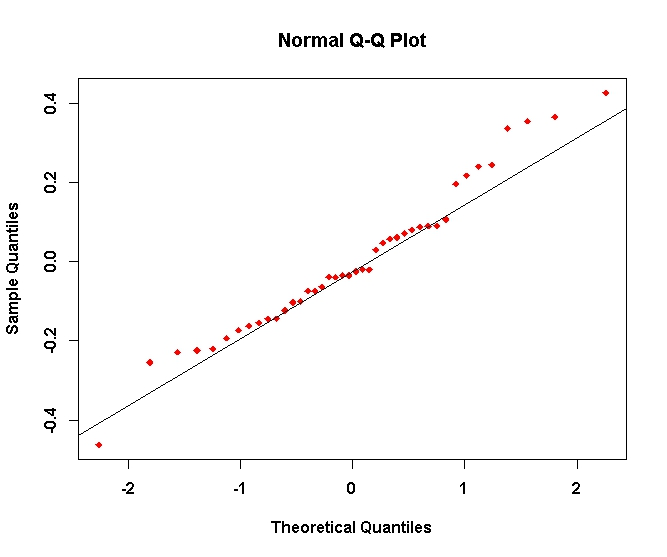
\includegraphics[scale=0.45]{images/ExamQ5qqplot}
\end{center}

\begin{itemize}
	\item[i.] (1 Mark) Provide a brief description on how to interpret this plot.
	\item[ii.] (1 Mark) What is your conclusion for this procedure? Justify your answer.
\end{itemize}

\subsection*{Q3. Testing Normality (4 Marks)} %4 Marks
Consider the following inference procedure performed on data set $X$.
\begin{center}
	\begin{verbatim}
> shapiro.test(X)

Shapiro-Wilk normality test

data:  X
W = 0.8914, p-value = 0.07047

	\end{verbatim}
\end{center}


\begin{itemize}
	\item[i.] (1 Mark) Describe what is the purpose of this procedure.
	\item[ii.] (1 Mark) What is the null and alternative hypothesis?
	\item[iii.] (1 Mark) Write the conclusion that follows from it.
	\item[iv.] (1 Mark) Tests for Normality are known to be susceptible to low power. Discuss what is meant by this.
\end{itemize}


\subsection*{Q4. Dixon Q Test For Outliers (4 Marks)}

The typing speeds for one group of 12 Engineering students were recorded both at the beginning of year 1 of their studies. The results (in words per minute) are given below:

\begin{center}
\begin{tabular}{|c|c|c|c|c|c|c|}
\hline
% Subject& A& B& C& D& E &F &G &H \\ \hline
121 & 146 & 150 &149 &142 &170& 153\\ \hline
 137 & 161 & 156& 165& 137& 178& 159
\\ \hline
\end{tabular}
\end{center}
Use the Dixon Q-test to determine if the lowest value (121) is an outlier. You may assume a significance level of 5\%.
%Calculate a 95\% confidence interval for the difference between the mean number of marks obtained by males and females in the population of school leavers as a whole.
%(7 marks)

\begin{itemize}
\item[i.] (1 Mark) Formally state the null hypothesis and the alternative hypothesis.
\item[ii.] (1 Mark) Compute the Test Statistic.
\item[iii.] (2 Mark) By comparing the Test Statistic to the appropriate Critical Value, state your conclusion for this test.
\end{itemize}


\subsection*{Q5. Testing For Outliers (6 Marks)}
\begin{itemize}
	\item[(i)] (3 Marks) Provide a brief description for three tests from the family of Grubb's  Outliers Tests. Include in your description a statement of the null and alternative hypothesis for each test, any required assumptions and the limitations of these tests.
	\item[(ii)] (3 Marks) Showing your working, use the Dixon Q Test to test the hypothesis that the maximum value of the following data set is an outlier.
	\[ 19,22,23,24,25,26,29,38\]
\end{itemize}

\newpage
\subsection*{Q6. Testing for Outliers (3 Marks)} %4 Marks
The following statistical procedure is based on this dataset.
\begin{center}
\begin{tabular}{|cccc|}
	\hline
	% after \\: \hline or \cline{col1-col2} \cline{col3-col4} ...
	6.98 &8.49 &7.97& 6.64\\
	8.80 &8.48 &5.94& 6.94\\
	6.89 &7.47 &7.32& 4.01\\
	\hline
\end{tabular}
\end{center}

\begin{framed}

	\begin{verbatim}
	> grubbs.test(x, two.sided=T)
	
	Grubbs test for one outlier
	
	data:  x
	G = 2.4093, U = 0.4243, p-value = 0.05069
	alternative hypothesis: lowest value 4.01 is an outlier
	\end{verbatim}
\end{framed}

\begin{itemize}
	\item[i.] (1 Mark) Describe what is the purpose of this procedure. State the null and alternative hypothesis.
	\item[ii.] (1 Mark) Write the conclusion that follows from it.
	\item[iii.] (1 Mark) State any relevant assumptions for this procedure.
\end{itemize}

\subsection*{Q7. Regression ANOVA}
%-------------------------------End  of Question 2A%
(4 Marks) Complete the following \textit{Analysis of Variance} Table for a simple linear regression model based on the data provided. The required values are indicated by question marks.
\begin{center}
	\begin{tabular}{|c|c|c|c|c|c|} \hline
		& DF & 	Sum Sq &	Mean Sq &	F value &   	Pr($>$F)    \\ \hline
		Regression &  ? &	9160239 &	? &	 ? &	$< 2.2e^{-16}$ \\ \hline
		Error  & 50 &	2134710 &  	?   &            &       \\ \hline
		Total  & ?  &	? &  	?  &            &       \\ \hline
	\end{tabular} 
\end{center}

Once you have completed this table, compute the following
\begin{itemize}
	\item (1 Mark) The Pearson correlation coefficient for the response variable Y and the predictor variable X.\textit{ (You may assume that the Pearson Correlation Coefficient is a positive number.)}
	\item (1 Mark) The sample standard deviation of the response variable Y.
\end{itemize}
\newpage
\subsection*{Q8. Regression ANOVA}
The mercury level of several tests of sea-water from costal areas was determined by atomic-absorption spectrometry. The results obtained are as follows

\begin{figure}[h!]
\centering
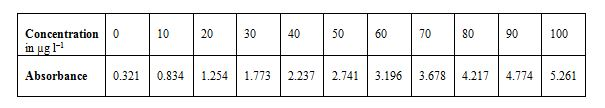
\includegraphics[width=1.1\linewidth]{image/regressionData}
\end{figure}

The analysis of the relationship between concentration and absorbance is obtained in R and presented below. 
\begin{framed}
\begin{verbatim}
x<-seq(0,100,by=10)
y<- c(0.321, 0.834, 1.254, 1.773, 2.237, 2.741, 3.196, 3.678, 
 4.217, 4.774, 5.261)
model<- lm(y~x)
summary(model)

Call:
lm(formula = y ~ x)

Coefficients:
            Estimate Std. Error t value Pr(>|t|)    
(Intercept) 0.2933636  0.0234754   12.50 5.45e-07 
x           0.0491982  0.0003968  123.98 7.34e-16 
---

Residual standard error: 0.04162 on 9 degrees of freedom
Multiple R-squared: 0.9994,     Adjusted R-squared: 0.9993 
F-statistic: 1.537e+04 on 1 and 9 DF,  p-value: 7.337e-16 

confint(model)
            2.5 %     97.5 %
(Intercept) 0.24025851 0.34646876
x           0.04830054 0.05009582

\end{verbatim}
\end{framed}

\begin{itemize}
\item[(i)] (2 marks)
Determine and interpret the slope and the intercept of the calibration plot.
\item[(ii)] State the 95\% confidence interval for the slope and the intercept coefficients. Interpret this intervals with respect to any relevant hypothesis tests
\item[(iii)] (2 marks) Explain in which way is the prediction intervals different from the confidence intervals for fitted values in linear regression?
\item[(iv)] (2 Marks) The following piece of \texttt{R} code gives us a statistical metric. What is this metric? What is it used for? How should it be interpreted.

\end{itemize}
\begin{framed}
	\begin{verbatim}
> AIC(model)
[1] -34.93389	
\end{verbatim}
\end{framed}
\subsection*{Q9. Robust Regression}

In certain circumstances, Robust Regression may be used in preference to Ordinary Least Squares Regression. 

Answer the following questions relating to Robust Regression. 

\begin{itemize}
	\item[(i)] (1 Mark) Describe what these circumstances might be.
	\item[(ii)] (1 Mark) State one difference between OLS and Robust regression techniques, in terms of computing regression equations.
	\item[(iii)] (2 Marks) Explain the process of Huber Weighting, stating the algorithm used to compute weightings.
	\item[(iv)] (2 Marks) Suppose that Huber Weigthing, with a tuning constanct of $k=13.45$ was applied to the observations 
	tabulated below. What would be the outcome of the procedure for each case. 
\end{itemize}
\begin{center}
	\begin{tabular}{|c|c|}
		\hline
		Observation & Residual \\ 
		$i$  & $e_i$ \\ \hline
		11 & -9.07 \\ \hline 
		14 & 14.54 \\ \hline
		18 & 22.91 \\ \hline
	\end{tabular} 
\end{center}

%=================================================================%
\subsection*{Q10. Method Comparison}
\begin{itemize}
	\item[(i)] (1 Mark) Write a brief note on the topic of method comparison studies.
	\item[(ii)] (1 Mark)Why are OLS regression models not suitable for Method Comparison.
	\item[(iii)] (1 Mark) Describe an alternative regression technique. Include in your answer any variants of the technique and any limitations of using those technique.
	
	\item[(iv)] (2 Marks) A Bland Altman Plot is a graphical technique used in Method Comparison. Sketch a Bland-Altman plot and discuss how the various components are calculated.
\end{itemize}
\subsection*{Q11. Experimental Design }

% Definitions
% One Way ANOVA
% Checking Assumptions

Explain the following terms in the context of experimental design
	\begin{itemize}
		\item[i.] (2 marks) levels of a factor.
		\item[ii.] (2 marks) randomized block design.
	\end{itemize}
	
	%==================================================================%
\subsection*{Q12. One-Way ANOVA } %4 Marks
Six analysts each made seven determinations of the paracetamol content of the same batch of tablets.
The results are shown in the table below. In the last two columns are the sample means and standard deviations for each sample.\\
\bigskip

	\begin{tabular}{|c|ccccccc|c|c|}
		\hline
		Group &  & &  &  &  &  &  & $\bar{X}$& $S_{X}$ \\ \hline
		A & 84.32 & 84.51 & 84.63 & 84.61 & 84.64 & 84.51 & 84.62 & 84.5486 & 0.1209 \\ \hline
		B & 84.24 & 84.25 & 84.41 & 84.13 & 84.00 & 84.30 & 84.02 & 84.1928 & 0.1416 \\ \hline
		C & 84.29 & 84.40 & 84.68 & 84.28 & 84.40 & 84.36 & 84.63 & 84.4342 & 0.1459 \\ \hline
		D & 84.14 & 84.22 & 84.02 & 84.48 & 84.27 & 84.33 & 84.22 & 84.2400 & 0.1583 \\ \hline
		E & 84.50 & 83.88 & 84.49 & 83.91 & 84.11 & 84.06 & 83.99 & 84.1343 & 0.2749 \\ \hline
		F & 84.70 & 84.17 & 84.11 & 84.36 & 84.61 & 83.81 & 84.15 & 84.2729 & 0.3324 \\ \hline
	\end{tabular} 
	


\bigskip
For the aggregrate sample (all 42 observations) the standard deviation is $0.2381$.

\begin{itemize}
	\item[(i)] (5 Marks) Complete the following One Way Analysis of Variance Table.
	\item[(ii)] (1 Marks) Describe what is the purpose of this procedure. include a statement of the null and alternative hypothesis in your answer.
%	\item[(iii)] (2 Marks) (5 Marks)
\end{itemize}
\begin{tabular}{|r|c|c|c|c|c|}
	\hline Source  &\phantom{sp} DF \phantom{sp} & Sum Squares & Mean Square  & \phantom{sp} F \phantom{sp} & p-value  \\ 
	\hline Between-Groups &  &  &  &  & 0.003941 \\ 
	\hline Within-Groups &  &  &  &  &  \\ \hline
	\hline Total &  &  &  &  &  \\ 
	\hline 
\end{tabular} 

%==================================================================%
\newpage
\subsection*{Q13. Testing assumptions for ANOVA } %4 Marks
The \texttt{R} code and graphical procedures, below and on the following page, are relevant to checking whether the underlying assumptions are met for the ANOVA model in part (b).
\begin{itemize}
	\item[i.] (3 marks) What are the assumptions underlying ANOVA?
	\item[ii.] (4 marks)  Assess the validity of these assumptions for the ANOVA model in part(b).
	
\end{itemize}
\begin{framed}
	\begin{verbatim}
	Shapiro-Wilk normality test
	
	data:  Residuals
	W = 0.9719, p-value = 0.3819
	\end{verbatim}
\end{framed}
\begin{framed}
	\begin{verbatim}
	Bartlett test of homogeneity of variances
	
	data:  Experiment
	Bartlett's K-squared = 105.9585, df = 1, p-value < 2.2e-16
	\end{verbatim}
\end{framed}
\begin{center}
	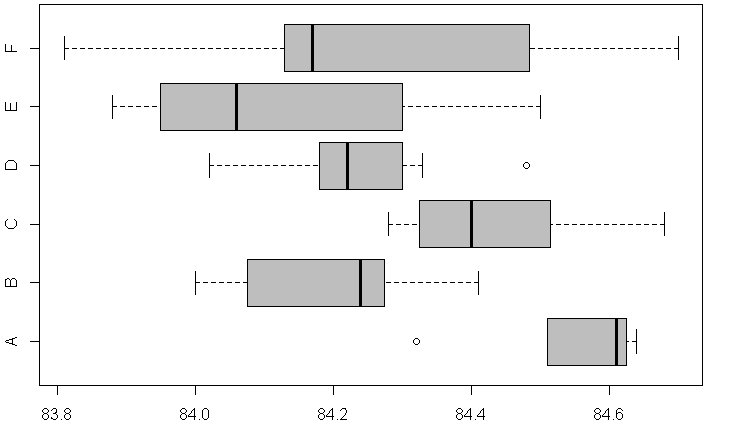
\includegraphics[scale=0.59]{images/ExamQ5boxplot}
\end{center}
\newpage
%qqnorm(resid(Model),pch=18,col="red",font.lab=2,font.axis=2)
%qqline(resid(Model))
\begin{center}
	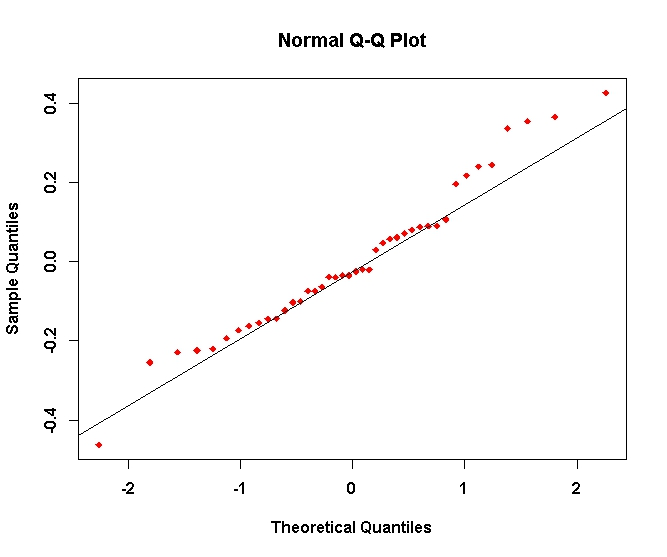
\includegraphics[scale=0.55]{images/ExamQ5qqplot}
\end{center}
\begin{center}
	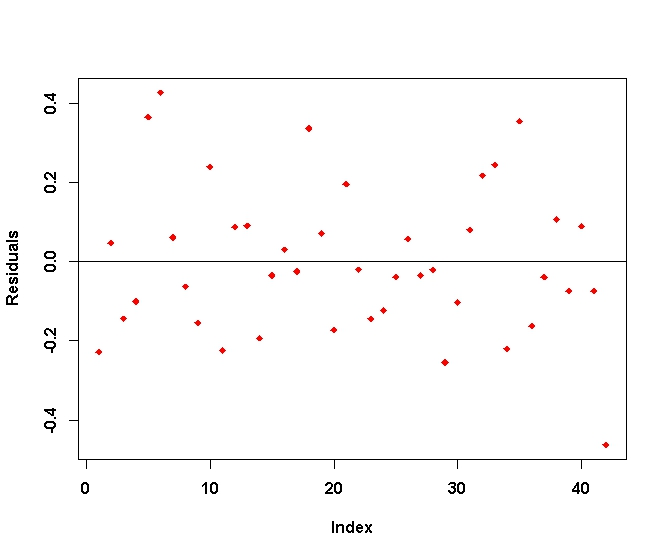
\includegraphics[scale=0.55]{images/ExamQ5resid}
\end{center}

\subsection*{Q14. ANOVA  Example }
	
	Assume that we have three fertilizers to be tested. We wish to determine if there is any difference is the mean yields for the three different types of fertilizer.
	\begin{center}
		\begin{tabular}{|c|c|c|c|c|}
			\hline
			Fertilizer	A	&	5.6	&	6.4	&	6.6	&	5.8	\\ \hline
			Fertilizer	B	&	5.1	&	6.2	&	6.4	&	5.7	\\ \hline
			Fertilizer	C	&	5.0	&	6.1	&	5.8	&	5.5	\\ \hline
		\end{tabular} 
	\end{center}
	The following \texttt{R} output is a One-Way ANOVA procedure for testing multiple means.
	
	\begin{framed}
		\begin{verbatim}
		Fert <- c("A", "A", "A", "A", "B", "B", "B", "B", 
		"C", "C", "C", "C")
		Yield <- c(5.6, 6.4, 6.6, 5.8, 5.1, 6.2, 6.4, 5.7, 
		5, 6.1, 5.8, 5.5)
		
		ModelA=aov(Yield~Fert)
		\end{verbatim}
	\end{framed}
	\begin{verbatim}
	> summary(aov(Yield~Fert))
	            Df Sum Sq Mean Sq F value Pr(>F)
	Fert         2   0.50  0.2500   0.957   0.42
	Residuals    9   2.35  0.2611 
	\end{verbatim}
	
\textbf{State you conclusion to this procedure}
\subsection*{Q15. Two Way ANOVA } 
\begin{itemize}
	\item A standard solution was prepared, containing 16.00\% (by weight) of chloride. Three titration methods, each with a different technique of end-point determination, were used to analyse the standard solution.
	\item The procedure was carried out by four different clinical analysts. The order of the experiments was randomized. The results for the chloride found (\% w/w) are shown below:
	
\end{itemize}

\begin{center}
	\begin{tabular}{|c|c|c|c|c|}
		\hline 	& Analyst 1	&Analyst 2	&Analyst 3	&Analyst 4	\\ \hline
		Method A	&	16.03	&	16.05	&	16.02	&	16.12	\\ \hline
		Method B	&	16.13	&	16.13	&	15.94	&	15.97	\\ \hline
		Method C	&	16.09	&	16.15	&	16.12	&	16.1	\\ \hline
	\end{tabular}
\end{center}

\begin{framed}
	\begin{verbatim}
	> Model=aov(Titr ~ Meth + Anlt) 
	> 
	> summary(Model) 
	Df  Sum Sq   Mean Sq  F value Pr(>F)    
	Meth           2  0.01202  0.006008 1.279   0.345  
	Anlt           3  0.01109  0.003697 0.787   0.543  
	Residuals      6  0.02818  0.004697   
	
	---
	Signif. codes:  0 ‘***’ 0.001 ‘**’ 0.01 ‘*’ 0.05 ‘.’ 0.1 ‘ ’ 1
	\end{verbatim}
\end{framed}

\textbf{State you conclusion to this procedure}
\subsection*{Q16. One Way ANOVA } 
Four laboratory technicians performed six determination of $C$ of 2,4 dinitrophenol in water, according to the same specified procedure.
The results in $C/ \mu M$ are as follows

\begin{center}
	\begin{tabular}{|c|c|c|c|}
		\hline Analyst A	&	Analyst B	&	Analyst C	&	Analyst D	\\ \hline
		701	&	550	&	511	&	613	\\ \hline
		677	&	545	&	523	&	623	\\ \hline
		680	&	573	&	540	&	649	\\ \hline
		660	&	532	&	542	&	632	\\ \hline
		654	&	529	&	559	&	614	\\ \hline
		648	&	534	&	554	&	626	\\ \hline
	\end{tabular} 
\end{center}
The analysis of variance procedure is used to determine
if there is a significiant difference between the mean of the
determinations makde by the four investigators.


\begin{framed}
	\begin{verbatim}
	summary(aov(Det~Anlt))
	            Df Sum Sq Mean Sq  F value   Pr(>F)    
	Anlt        ..  99942   ....    .....    4.64e-12 ***
	Residuals   ..   6918   ....                     
	---
	Signif. codes:  0 ‘***’ 0.001 ‘**’ 0.01 ‘*’ 0.05 ‘.’ 0.1 ‘ ’ 1
	\end{verbatim}
\end{framed}

\begin{itemize}
	\item[(a)] The value for the degrees of freedom for residuals has been removed from the output. What is this value?
	\item[(b)] The value for the test statistics (\texttt{F value}) has been removed from the output. What is this value?
	\item[(c)] State the null and alternative hypothesis for this procedure.
	\item[(d)] Based on the $p-$value, what is your conclusion for this procedure.
\end{itemize}


%==================================================================%
\subsection*{Q17. Two Way ANOVA } %4 Marks
Four standard solutions of chloride were prepared. Three titration methods, each with a different technique of end-point determination, were used to analyze each standard solution. The order of the experiments was randomized. The results of chloride found are shown below.
\begin{figure}[h!]
\centering
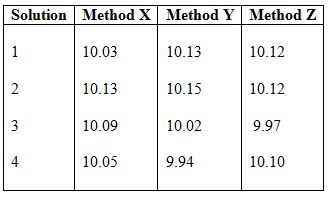
\includegraphics[width=0.5\linewidth]{image/TwoWayANOVAdata}

\end{figure}
\noindent The following output table is the result of performing a two-way ANOVA (without
interactions). \\

\bigskip
\noindent \textbf{Analysis of Variance Table}
\begin{framed}
	{
		\Large
\begin{verbatim}
Response: chloride

          Df   Sum Sq   MeanSq  F value    Pr(>F)
A          ? 0.011092 	 ?       0.7871    0.5435
B          ? 0.012017 	 ?       1.2791    0.3446
Residuals  ? 0.028183   ?      
Total      ?        ?              
\end{verbatim}
}
\end{framed}

\begin{itemize}
\item[(a)]	Identify the two factors A and B, and their corresponding levels. Are they controllable or random? Construct the hypothesis statements.
(2 marks)
\item[(b)]	 Fill in the missing values for the mean sum of squares.
(2 marks)
\item[(c)]	Test whether there are significant differences between the concentration of chloride in the different solutions, and whether there are significant differences between the results obtained by the different methods.
(2 marks)
\item[(d)]	Compute the variance of the all results computed for this experiment.
(2 marks)
\item[(e)]	Is it possible to include the interaction term in the model, given the data we have? Why? How can this be changed?
(2 marks)
\end{itemize}

%==================================================================%
\subsection*{Q18. Residual Analysis for Regression Models} %4 Marks
Explain the following terms
\begin{itemize}
\item[(i)]	Influence
\item[(ii)]	Leverage
\item[(iii)]	Cook’s Distance
\end{itemize}
Write a brief explanation of how robust regression differs from linear models computed using the \textbf{\textit{Ordinary Least Squares}} method, making reference to one particular weighting method.


%==================================================================%

\subsection*{Q19. Numeric Transformation of Data} %4 Marks


\begin{itemize}
	\item[(i)] Describe the purpose of transformations
	\item[(ii)] Describe the process of transformations
	\item[(iii)] Describe the purpose of Tukey's Ladder (referencing direction and relative strength)
	\item[(iv)] Give an example of a transformation for various types of skewed data (use Tukey's Ladder, with an example for both directions)
	\item[(v)] Describe the limitations of transformations
\end{itemize}

\subsection*{Q20. Inference Procedures with \texttt{R}} %4 Marks
\begin{figure}[h!]
\centering
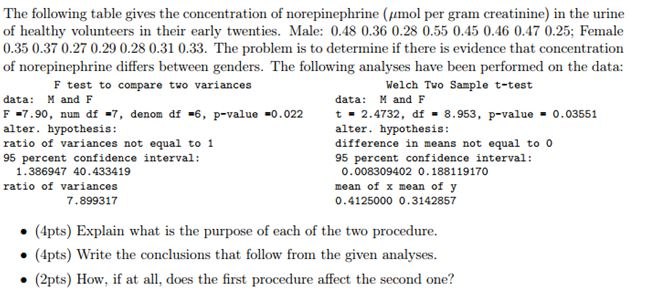
\includegraphics[width=1.1\linewidth]{image/Q20REview}
\end{figure}
\newpage
\subsection*{Q21. Inference Procedures with \texttt{R}} %4 Marks
\begin{figure}[h!]
\centering
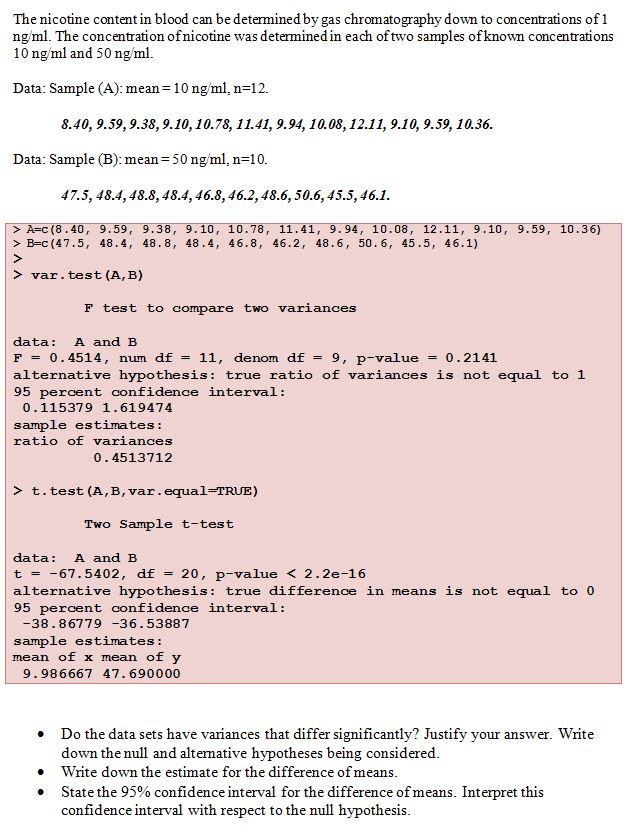
\includegraphics[width=0.95\linewidth]{image/Q21review}

\end{figure}
\newpage
\subsection*{Q22. Two Way ANOVA - No Replicates} %4 Marks

Three varieties of potatoes are being compared for yield. The experiment
was carried out by assigning each variety at random to four of twelve equal size
plots, one being chosen in each of four locations. The following yields in bushels per 
plot resulted:
% A bushel is about 36.4 litres.

\begin{figure}[h!]
	\centering
	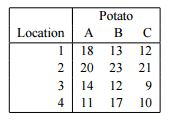
\includegraphics[width=0.4\linewidth]{twowayanova-potato}
\end{figure}
\noindent \textbf{Additional Information} 

\begin{itemize}
	\item The variance of the Row means is : $S^2_{R} = 19.037$. 
	\item the variance of the Column means is : $S^2_{C} = 3.0625$.	
	\item Also the overall variance of the 12 observations is $\textrm{Var}(Y) = 21.6363 $. 
\end{itemize}

\noindent \textbf{Exercise} Complete the Two Way ANOVA table. You are not required to perform any hypothesis testing.
\newpage
\subsection*{Q23. One Way ANOVA } %4 Marks


\begin{figure}[h!]
\centering
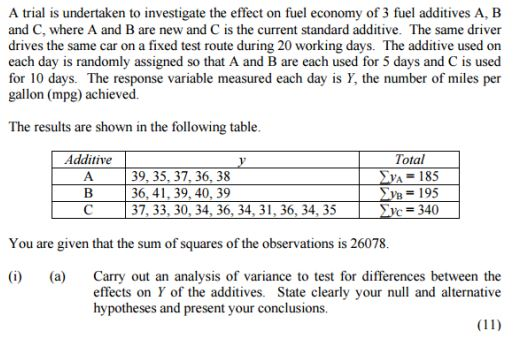
\includegraphics[width=1.1\linewidth]{image/Q23Review}
\end{figure}
You are given the additional piece of information , sufficient to construct ANOVA table

{
\Large
\begin{center}
\begin{tabular}{|c|c|c|c||c|} 
	\hline  & A & B & C & Overall \\ 
	\hline Mean & 37 & 39& 34 &36 \\ 
	\hline Std.Dev &  1.5811 & 1.8708 & 2.2111 & 2.8837 \\
	
	\hline 
\end{tabular}
\end{center}
}
The p-value for the Test Statistic is 0.00650

\newpage
\subsection*{Q24. Two Way ANOVA }
Given the following details below, construct the appropriate Two-Way ANOVA Table. \textit{You are not required to do any hypothesis testing.}

\begin{itemize}
	\item There are 2 factors: A and B. A has 2 levels, while Factor B has 3 levels.
	\item There are 54 observations in the experiment.
	\item The variance of the response variable is 174.2075.
	\item The Sum of Squares for Factors A and B are 451  and  2034 respectively.
	\item The Sum of Squares for Error is 5745.
\end{itemize}


\newpage

\subsection*{Q25. One Way ANOVA }
\begin{figure}[h!]
	\centering
	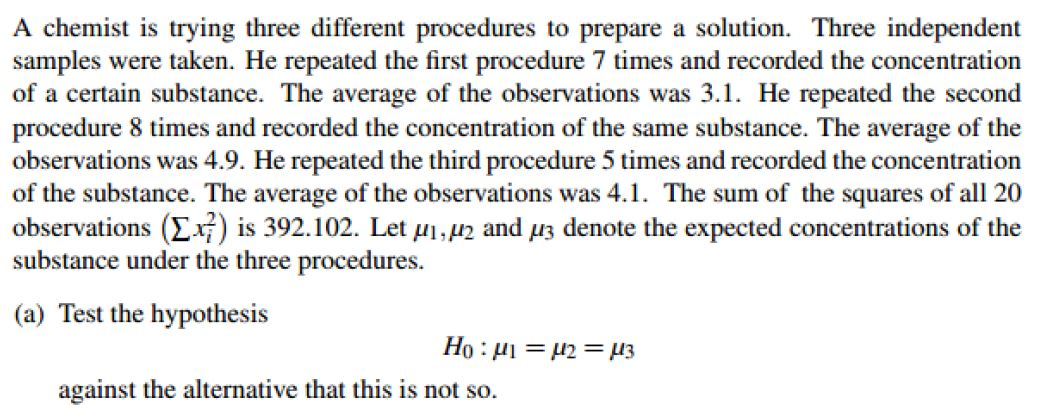
\includegraphics[width=0.7\linewidth]{image/Q24review1}
	
\end{figure}

\noindent \textbf{Additional Information: }
\begin{itemize}
	\item The Variance of the Response Variable is 3.2. (You can ignore the part about “the sum of squares for all 20 obervations”.)
	\item  Ordinarily you would be given the standard deviation for each sample, and from that, directly compute SSwithin. In this question , use this identity : SStotal = SSbetween + SSwithin.
	\item  You have been given enough information to compute the Overall Mean.
	\item  We may not get around to covering the confidence intervals material in MA4605 2015. It will be retained for possible use in future.
\end{itemize}
\newpage
\subsection*{Q26. Two Way ANOVA (no replicates)}
\begin{figure}[h!]
	\centering
	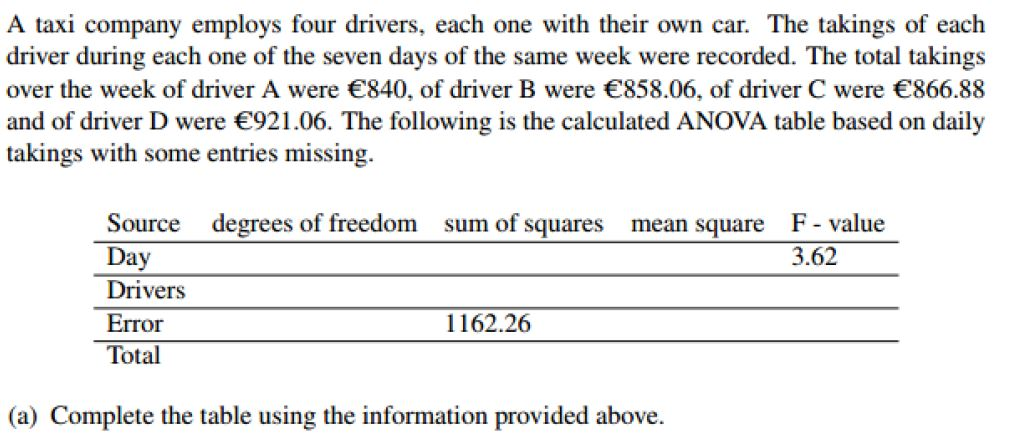
\includegraphics[width=0.8\linewidth]{image/Q26Review1}
	
\end{figure}
\begin{figure}[h!]
	\centering
	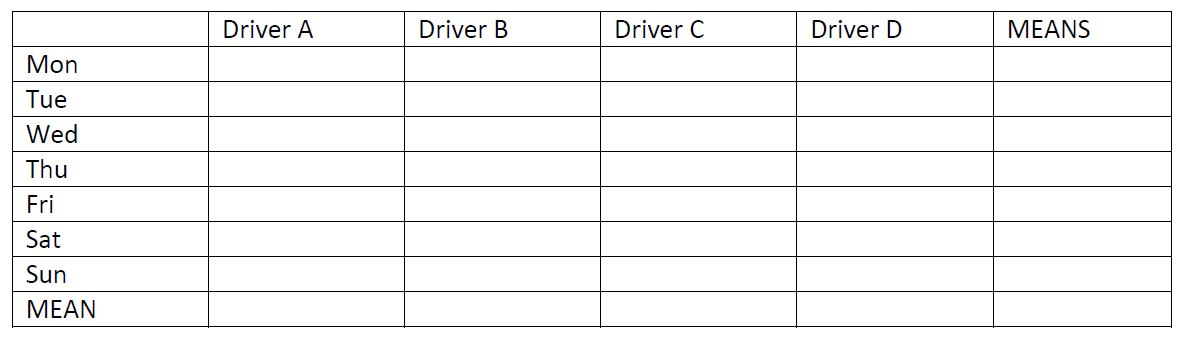
\includegraphics[width=0.8\linewidth]{image/Q26review2}
	
\end{figure}
\begin{figure}[h!]
	\centering
	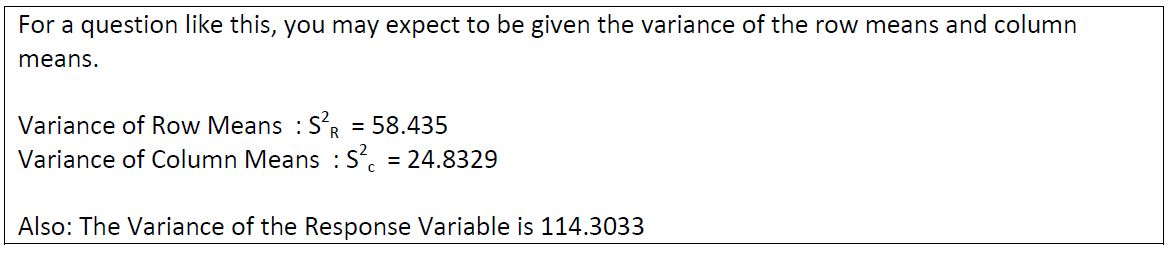
\includegraphics[width=0.8\linewidth]{image/Q26review3}
	
\end{figure}
\newpage
\subsection*{Q27. One Way ANOVA }
\begin{figure}[h!]
	\centering
	\includegraphics[width=0.7\linewidth]{image/Q27review1}
	
\end{figure}
\noindent \textbf{Additional Information: }
\begin{itemize}
	\item The variance of the response variable is 831.3695. (\textit{You can ignore now some of the information given in the question}) 
	\item  In this question , use this identity : SStotal = SSbetween + SSwithin.
	\item  You have been given enough information to compute the Overall Mean.
	\item  We may not get around to covering the confidence intervals material in MA4605 2015. It will be retained for possible use in future.
\end{itemize}
\newpage
\subsection*{Q28. Two Way ANOVA (no replicates)}
\begin{figure}[h!]
	\centering
	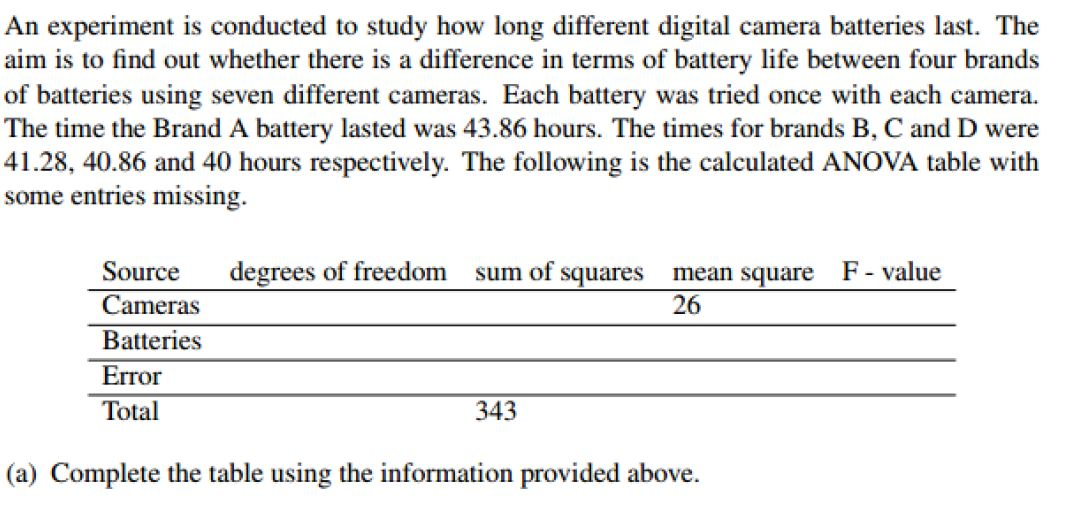
\includegraphics[width=0.9\linewidth]{image/Q28Review1}
	
\end{figure}
\begin{figure}[h!]
	\centering
	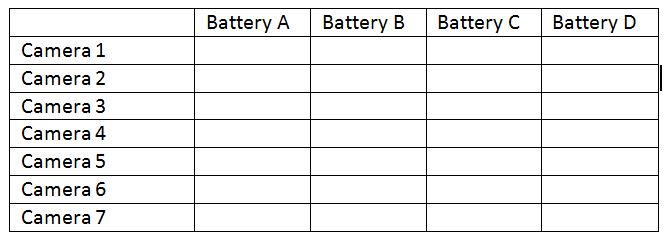
\includegraphics[width=0.9\linewidth]{image/Q28Review3}
	
\end{figure}
\begin{figure}[h!]
	\centering
	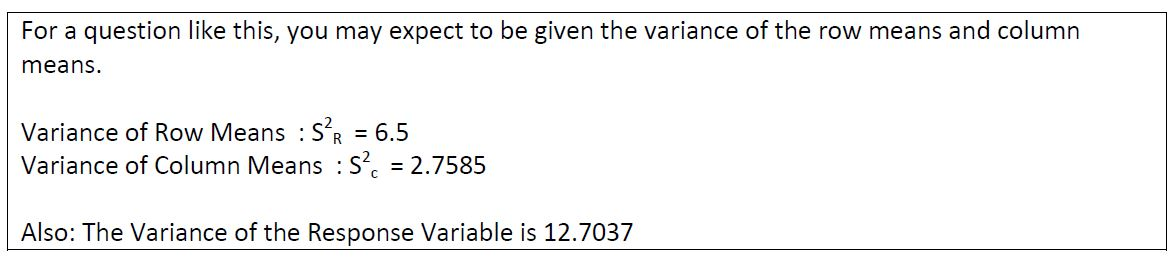
\includegraphics[width=0.9\linewidth]{image/Q28Review2}
	
\end{figure}
\newpage
\subsection*{Q29. Two Way ANOVA (with replicates)}

Consider the following experiment (similar to question 28) where there are 5 measurements per treatment group.
\begin{figure}[h!]
	\centering
	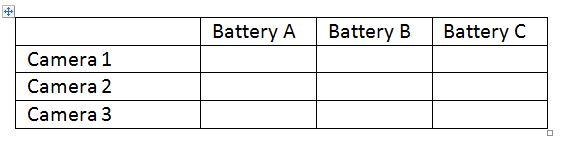
\includegraphics[width=0.8\linewidth]{image/Q29Review}
\end{figure}
Complete the following ANOVA table.\\ \bigskip
\begin{figure}[h!]
	\centering
	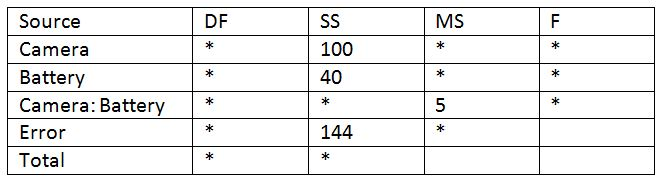
\includegraphics[width=0.8\linewidth]{image/Q29Review2}
\end{figure}\\


For the three F test statistics, state the appropriate degrees of freedom for the corresponding critival value. \textit{(You are not required to perform the hypothesis test)}
\newpage
\subsection*{Question 30 - Residual Diagnostics}
Expect a question on Hypothesis Tests from car \texttt{R} package, and Model diagnostic plots. This scope of this question covers the following topics.
\begin{itemize}
	\item \texttt{ncvTest()} - Non Constant Error Variance
	\item \texttt{outlierTest()} - Outliers
	\item \texttt{durbinWatsonTest()}  - Autocorrelation
	\item Cook's Distances
	\item Diagnostic Plot 1 (Fitted Vs Residual)
	\item Diagnostic Plot 2 (Residual Normality) 
\end{itemize}
\newpage
\subsection*{Question 31 - Control Limits }
\begin{figure}[h!]
\centering
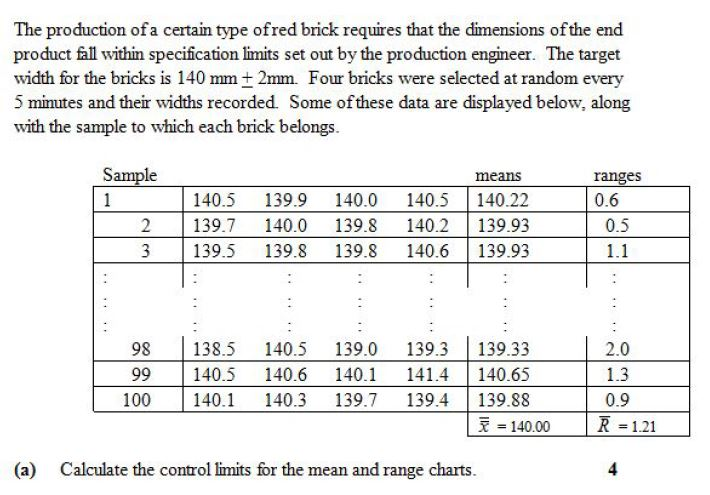
\includegraphics[width=1.1\linewidth]{images/ReviewQ31}

\end{figure}
The mean of the process standard deviations is $\bar{s} =0.2$.
\begin{framed}
	Exam Paper Formulas for Control Limits
	\begin{itemize}
		\item Process Mean
		
		
		
		\[ \bar{\bar{x}} \pm 3\frac{\bar{s}}{c_4\sqrt{n}}\]
		\item Process Standard Deviation	
		\[ \bar{s} \pm 3\frac{c_5\bar{s}}{c_4}\]
		\item Process Range	
		\[\left[ \bar{R}D_3, \bar{R}D_4\right]\]
	\end{itemize}	
\end{framed}
\newpage
\subsection*{Question 32 - Method Comparison}

An ion-selective electrode (ISE) determination of sulphide from sulphate-reducing bacteria was compared with a gravimetric determination. Each pair of determinations were taken from the same sample. \\ \\The results obtained by both methods are expressed in milligrams of sulphide, and are tabulated below.
\begin{center}
	\begin{tabular}{|c|cccccccccc|}
		\hline
		% after \\: \hline or \cline{col1-col2} \cline{col3-col4} ...
		ISE method & 108 & 12& 152 & 3 & 106 & 11 &  128 & 12& 160& 128 \\
		gravimetry & 105 & 16& 113 & 1 & 108 &  11 & 141 & 161 & 182& 118\\
		\hline
	\end{tabular}
\end{center}
Two simple linear models are fitted to the data. Model C uses the gravimetric determination as an independent variable used to predict the ISE determination. Conversely, Model D uses the ISE determination as an independent variable used to predict the gravimetric determination. The relevant \texttt{R} output is presented on the following page.
%Method Comparison Studies

\begin{itemize}
	\begin{framed}
		\item \textbf{Model C}
		\begin{verbatim}
		Call:
		lm(formula = ISE ~ grav)
		...
		Coefficients:
		Estimate Std. Error t value Pr(>|t|)
		(Intercept)  15.1125    28.8487   0.524    0.615
		grav          0.6997     0.2543   2.751    0.025 *
		....
		\end{verbatim}
	\end{framed}
	\begin{framed}
		\item \textbf{Model D}
		\begin{verbatim}
		Call:
		lm(formula = grav ~ ISE)
		..
		Coefficients:
		Estimate Std. Error t value Pr(>|t|)
		(Intercept)  38.6215    25.8542   1.494    0.174
		ISE           0.6949     0.2526   2.751    0.025 *
		....
		\end{verbatim}
	\end{framed}
\end{itemize}

\begin{itemize}
	%\item[i.] (4 marks) Write the regression equation for both of the fitted models.
	\item[i.] (3 marks) Is a simple linear regression model an suitable approach for this type of analysis? Explain why or why not? What alternative type of regression analysis might you recommend?
	\item[ii.] (2 marks) Provide a brief description of the Bland-Altman plot. Discuss any shortcomings with this approach to method comparison.
\end{itemize}


\subsection*{Question 33 - Inference Procedures}
\begin{itemize}
	\item The nicotine content in blood can be determined by gas chromatography down to concentrations of 1 ng/ml. The concentration of nicotine was determined in each of two samples of known concentrations 10 ng/ml and 50 ng/ml.
	\begin{framed}
		\begin{verbatim}
		Data: Sample (Lo): m = 10 ng/ml, n=14.
		
		8.40, 9.59, 9.38, 9.10, 10.78, 11.41, 9.94, 
		10.08, 12.11, 9.10, 9.59, 10.36, 10.41, 10.52.
		
		Data: Sample (Hi): m = 50 ng/ml, n=10.
		
		47.5, 48.4, 48.8, 48.4, 46.8, 
		46.2, 48.6, 50.6, 45.5, 46.1.
		\end{verbatim}
	\end{framed}
	A research team evaluated both samples to determine whether or not the samples were similar in terms of measures of centrality and dispersion, before the trial commenced.  \\  \\ The following blocks of \texttt{R} code (i.e blocks 1 to 6) are based on the data for this assessment. \\ 
	\begin{itemize}
		\item[(a)] (10 Marks) Each of the six blocks of code describes a statistical inference procedure. Provide a brief description for each procedure.
		\item[(b)] (10 Marks) Write a short report on your conclusion for this assessment, clearly indicating which blocks of \texttt{R} code you felt were most relevant, and explain why. 
	\end{itemize}
	
	\begin{itemize}
		\item[\textbf{Block 1}]
		\begin{framed}
			\begin{verbatim}
			
			F test to compare two variances
			
			data:  Lo and Hi
			F = 0.3945, num df = 13, denom df = 9, p-value = 0.1246
			alternative hypothesis: 
			true ratio of variances is not equal to 1
			95 percent confidence interval:
			0.1029905 1.3066461
			sample estimates:
			ratio of variances 
			0.3945149
			\end{verbatim}
		\end{framed}
		\newpage
		\item[\textbf{Block 2}]
		\begin{framed}
			\begin{verbatim}
			> shapiro.test(Lo)
			
			Shapiro-Wilk normality test
			
			data:  Lo
			W = 0.9779, p-value = 0.9609
			> shapiro.test(Hi)
			
			Shapiro-Wilk normality test
			
			data:  Hi
			W = 0.9496, p-value = 0.6634
			\end{verbatim}
		\end{framed}
		\bigskip
		\item[\textbf{Block 3}]
		\begin{framed}
			\begin{verbatim}
			> t.test(Lo,Hi)
			
			Welch Two Sample t-test
			
			data:  Lo and Hi
			t = -67.374, df = 14.016, p-value < 2.2e-16
			alternative hypothesis: 
			true difference in means is not equal to 0
			95 percent confidence interval:
			-38.83294 -36.43706
			sample estimates:
			mean of x mean of y 
			10.055    47.690 
			\end{verbatim}
		\end{framed}
		
		\item[\textbf{Block 4}]
		\begin{framed}
			\begin{verbatim}
			> t.test(Lo,Hi,var.equal=TRUE)
			
			Two Sample t-test
			
			data:  Lo and Hi
			t = -72.6977, df = 22, p-value < 2.2e-16
			alternative hypothesis: 
			true difference in means is not equal to 0
			95 percent confidence interval:
			-38.70863 -36.56137
			sample estimates:
			mean of x mean of y 
			10.055    47.690 
			
			\end{verbatim}
		\end{framed}
		
		
		
		\item[\textbf{Block 5}]
		\begin{framed}
			\begin{verbatim}
			> ks.test(Lo,Hi)
			
			Two-sample Kolmogorov-Smirnov test
			
			data:  Lo and Hi
			D = 1, p-value = 1.02e-06
			alternative hypothesis: two-sided
			
			\end{verbatim}
		\end{framed}
		%------------------------------------------------------------------%
		\item[\textbf{Block 6}]
		\begin{framed}
			\begin{verbatim}
			wilcox.test(Lo,Hi)
			
			Wilcoxon rank sum test
			
			
			data:  Lo and Hi
			W = 0, p-value = 1.02e-06
			alternative hypothesis: 
			true location shift is not equal to 0
			
			\end{verbatim}
		\end{framed}
	\end{itemize}
	
\end{itemize} % End of Question Block

%=============================================================================== %
\subsection*{Question 34 - Experimental Design}
\textit{(Remark : This question will not feature in the 2015 Winter Exam)}
\begin{itemize}
	\item[(i)] Give the principal features of a  balanced completely randomised design, and
	explain the role of replication in such a design.  \item[(ii)] State the statistical model for
	this design, define the terms in the model and state the standard assumptions
	made about the error term.
	\item[(iii)] Two basic principles of experimental design are \textbf{randomisation} and
	\textbf{replication}. Explain why these are important and how they help to
	validate an analysis of experimental results. 
	\item[(iv)] Briefly explain the principles of randomisation and replication, in the
	context of a completely randomised experimental design. Write down the model equation for a completely randomised design
	having equal numbers of replicates in all treatment groups, defining all
	the symbols that you use.
\end{itemize}
%================================== %
\subsection*{Question 35 - (NOT USING)}
Short Experimental Design Theory Question
\begin{itemize}
	\item Short Description on Box-Behnken Design
	\item Short Description on Central Composite Design
	\item Rationale for Designs like these
\end{itemize}
\textbf{Update:} This will not feature as a question in the Winter 2015 Exam.
\subsection*{Question 36-  Experimental Design Part 2 }

In an investigation into the extraction of nitrate-nitrogen from air dried soil, three quantitative variables were investigated at two levels. These were the amount of oxidised activated charcoal (A) added to the extracting solution to remove organic interferences, the strength of CaSO4 extracting solution (C), and the time the soil was shaken with the solution (T). The aim of the investigation was to optimise the extraction procedure. The levels of the variables are given here:
\begin{center}
	{
		\large
		\begin{tabular}{|cc|c|c|}
			\hline	&		&\phantom{sp}	{\LARGE -}\phantom{sp}	&	\phantom{sp} {\LARGE +} \phantom{sp}	\\ \hline
			Activated charcoal (g) 	&	A 	&	0.5	&	1	\\ \hline
			CaSO{4} (\%) 	&	C 	&	0.1	&	0.2	\\ \hline
			Time (minutes) 	&	T 	&	30	&	60	\\ \hline
		\end{tabular} 
	}
\end{center}

The concentrations of nitrate-nitrogen were determined by ultra-violet spectrophotometry and compared with concentrations determined by a standard technique. The results are given below and are the amounts recovered (expressed as the percentage of known nitrate concentration).
{
	\large
	\begin{center}
		\begin{tabular}{|c|c|c|cc|}
			\hline
			\phantom{sp}A\phantom{sp}	&	\phantom{sp}C\phantom{sp}	&\phantom{sp}	T\phantom{sp}	&	Amounts&	(2 Replicates)	\\
			\hline
			-1	&	-1	&	-1	&	45.1	&	44.6	\\ \hline
			
			1	&	-1	&	-1	&	44.9	&	45.3	\\ \hline
			
			-1	&	1	&	-1	&	44.8	&	46.7	\\ \hline
			
			1	&	1	&	-1	&	44.7	&	44.8	\\ \hline
			
			-1	&	-1	&	1	&	33	&	35	\\ \hline
			
			1	&	-1	&	1	&	53.8	&	51.7	\\ \hline
			
			-1	&	1	&	1	&	32.6	&	33.7	\\ \hline							
			1	&	1	&	1	&	54.2	&	53.2	\\ \hline
		\end{tabular}
	\end{center}
}



\newpage


\begin{itemize}
	\item[i.] (8 Marks) Calculate the contrasts, the effects and the sum of squares for the effects.
	\item[ii.] (8 Marks) Using the computed sums of squares values, complete the ANOVA table (see the \texttt{R} code below).
	\item[iii.] (4 Marks) Comment on the tests for significant for the main effects and interactions. State clearly your conclusions.
	\item[iv.] (4 Marks) Write down a  regression equation that can be used predicting amounts based on the results of this experiment.
\end{itemize}

\begin{framed}
	\begin{verbatim}
	Df Sum Sq Mean Sq F value     Pr(>F)    
	A            1    ...     ...     ...   0.000979 ***
	C            1    ...     ...     ...   0.934131    
	T            1    ...     ...     ...   0.395554 
	A:C          1    ...     ...     ...   0.944243    
	A:T          1    ...     ...     ...   0.017582 *
	C:T          1    ...     ...     ...   0.072101
	A:C:T        1    ...     ...     ...   0.028522 *    
	Residuals    8  116.2    14.5                      
	\end{verbatim}
\end{framed}

%\newpage
%\begin{center}
%	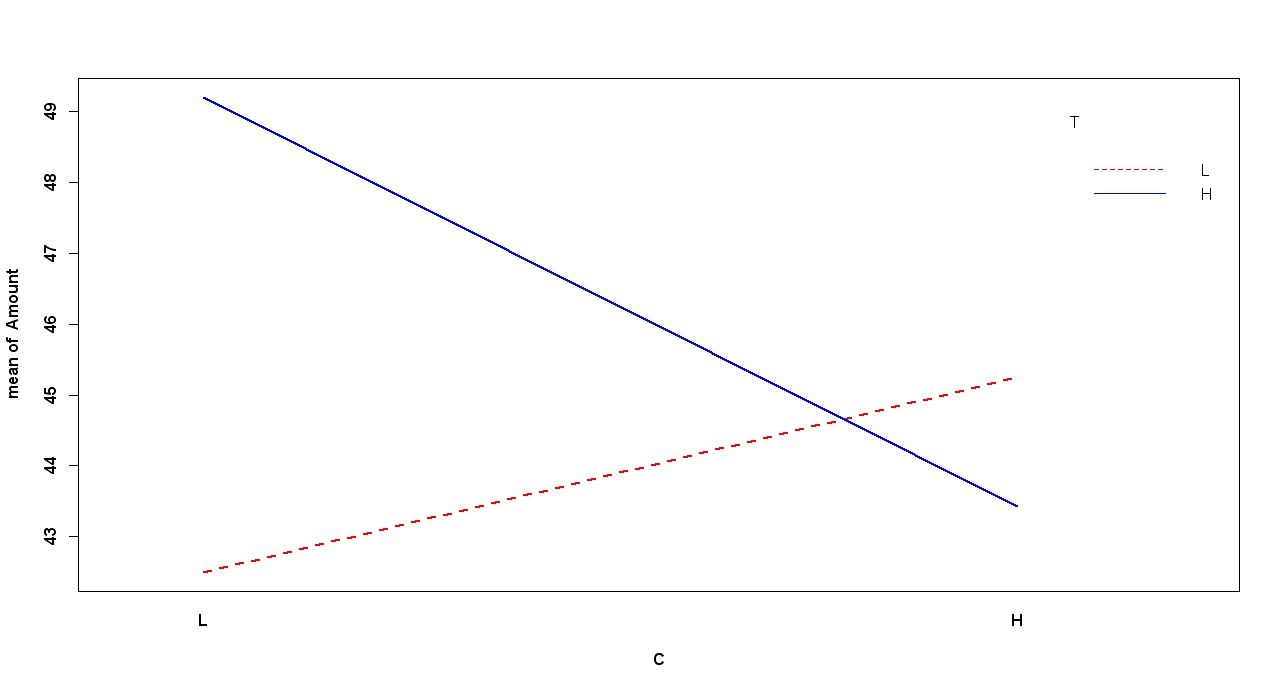
\includegraphics[scale=0.3]{images/ExamQ6interactionanew}
%\end{center}
%\begin{center}
%	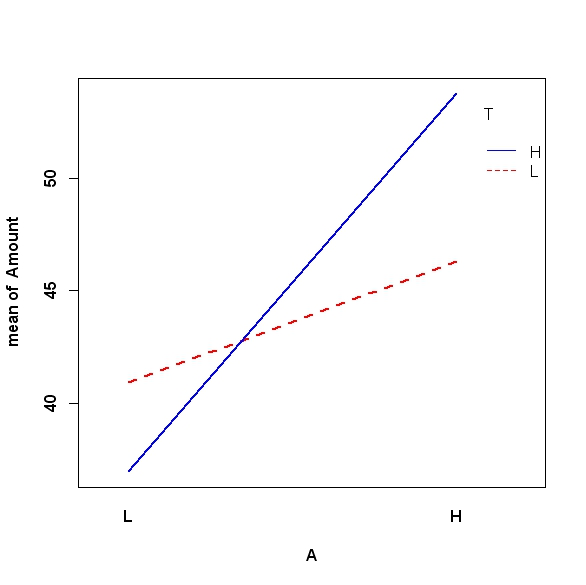
\includegraphics[scale=0.3]{images/ExamQ6interactionbnew}
%\end{center}
%\begin{center}
%	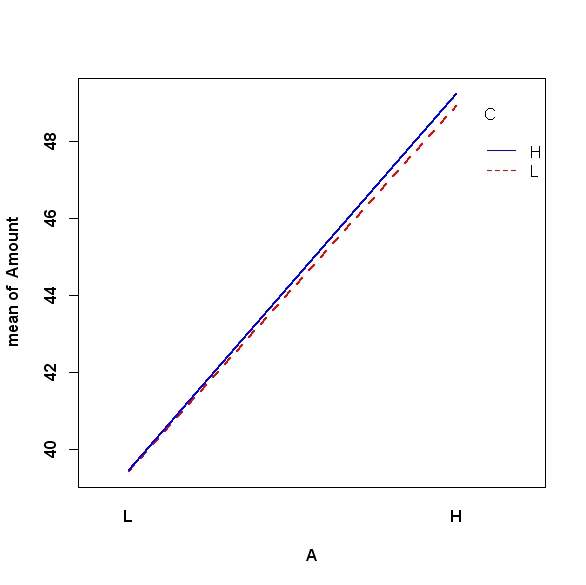
\includegraphics[scale=0.3]{images/ExamQ6interactioncnew}
%\end{center}

%================================================================ %
\newpage

\subsection*{Question 37 - ANOVA} Six analysts each made seven determinations of the paracetamol content of the same batch of tablets.
The results are shown below. There are 42 determinations in total. The mean determination for each analysts is also tabulated. \\


%Analyst= structure(c(1L, 2L, 3L, 4L, 5L, 6L, 1L, 2L, 3L, 4L, 5L, 6L, 1L,
%2L, 3L, 4L, 5L, 6L, 1L, 2L, 3L, 4L, 5L, 6L, 1L, 2L, 3L, 4L, 5L,
%6L, 1L, 2L, 3L, 4L, 5L, 6L, 1L, 2L, 3L, 4L, 5L, 6L), .Label = c("A",
%"B", "C", "D", "E", "F"), class = "factor")

%Determinations= c(84.32, 84.24, 84.29, 84.14, 84.5, 84.7, 84.61, 84.13, 84.28,
%84.48, 83.91, 84.36, 84.64, 84, 84.4, 84.27, 84.11, 84.61, 84.62,
%84.02, 84.63, 84.22, 83.99, 84.15, 84.51, 84.25, 84.4, 84.22,
%83.88, 84.17, 84.63, 84.41, 84.68, 84.02, 84.49, 84.11, 84.51,
%84.3, 84.36, 84.33, 84.06, 83.81)

\begin{center}
	\begin{tabular}{|c|ccccccc|}
		\hline
		Analyst	& Content		&		&		&		&		&		&		 \\ \hline
		A	&	84.32	&	84.61	&	84.64	&	84.62	&	84.51	&	84.63	&	84.51	 \\
		B	&	84.24	&	84.13	&	84.00	&	84.02	&	84.25	&	84.41	&	84.30	 \\
		C	&	84.29	&	84.28	&	84.40	&	84.63	&	84.40	&	84.68	&	84.36	 \\
		D	&	84.14	&	84.48	&	84.27	&	84.22	&	84.22	&	84.02	&	84.33	 \\
		E	&	84.50	&	83.91	&	84.11	&	83.99	&	83.88	&	84.49	&	84.06	 \\
		F	&	84.70	&	84.36	&	84.61	&	84.15	&	84.17	&	84.11	&	83.81	 \\
		\hline
	\end{tabular}
\end{center}
\bigskip
The following \texttt{R} output has been produced as a result of analysis of these data:

%Experiment=data.frame(Determinations, Analyst)
%Model=aov(Determinations~Analyst)
%summary(Model)

%Analysis of Variance Table
%
%            Df Sum Sq Mean Sq F value  Pr(>F)
%Analyst      5 0.8611 0.17222   4.236 0.00394 **
%Residuals   36 1.4635 0.04065
%---
%Signif. codes:  0 ‘***’ 0.001 ‘**’ 0.01 ‘*’ 0.05 ‘.’ 0.1 ‘ ’ 1

\begin{center}
	\texttt{
		\begin{tabular}{|c|cccccc|}
			\hline
			% after \\: \hline or \cline{col1-col2} \cline{col3-col4} ...
			&&		&		&		&		&		\\
			Response: Y        	&&	Df  	&	Sum Sq 	&	Mean Sq 	&	F value    	&	$Pr(>F)$    	\\
			&&		&		&		&		&		\\\hline
			&&		&		&		&		&		\\
			Analyst 	&&	\textbf{?}	&	\textbf{?}	&	\textbf{?}	&	\textbf{?}	&	0.00394 **	\\
			&&		&		&		&		&		\\ \hline
			&&		&		&		&		&		\\
			Residuals	&&	\textbf{?}	&	\textbf{?}	&	0.04065	&	&		\\
			&&		&		&		&		&		\\ \hline
			&&		&		&		&		&		\\
			Total	&&	\textbf{?}	&	2.3246	&		&		&		\\
			&&		&		&		&		&		\\ \hline
		\end{tabular}
	}
\end{center}
\begin{itemize}
	\item[i.] (5 marks) Complete the ANOVA table in your answer sheet, replacing the "?" entries with the correct values.
	\item[ii.] (2 marks) What hypothesis is being considered by this procedure.
	\item[iii.] (2 marks) What is the conclusion following from the above analysis? State the null and alternative hypothesis clearly.
\end{itemize}
\newpage


\subsection*{Question 38 - Assumptions for ANOVA}

The \texttt{R} code and graphical procedures, below and on the following page, are relevant to checking whether the underlying assumptions are met for the ANOVA model in part (b).
\begin{itemize}
	\item[i.] (3 marks) What are the assumptions underlying ANOVA?
	\item[ii.] (4 marks)  Assess the validity of these assumptions for the ANOVA model in the previous question (Question 37).
	
\end{itemize}
\begin{framed}
	\begin{verbatim}
	Shapiro-Wilk normality test
	
	data:  Residuals
	W = 0.9719, p-value = 0.3819
	\end{verbatim}
\end{framed}
\begin{framed}
	\begin{verbatim}
	Bartlett test of homogeneity of variances
	
	data:  Experiment
	Bartlett's K-squared = 105.9585, df = 1, p-value < 2.2e-16
	\end{verbatim}
\end{framed}
\begin{center}
	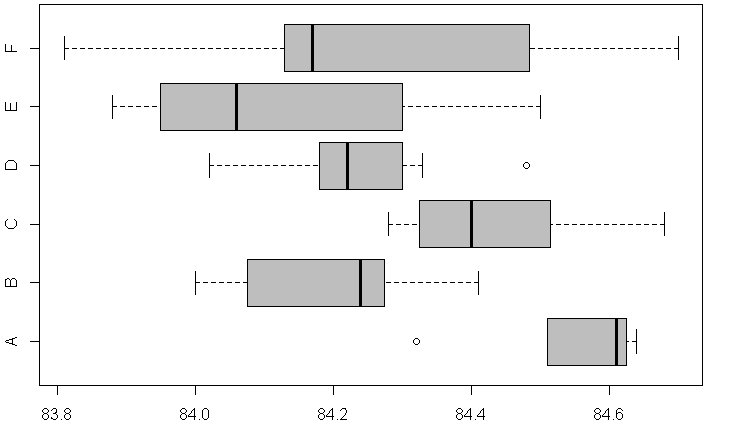
\includegraphics[scale=0.59]{images/ExamQ5boxplot}
\end{center}
\newpage
%qqnorm(resid(Model),pch=18,col="red",font.lab=2,font.axis=2)
%qqline(resid(Model))
\begin{center}
	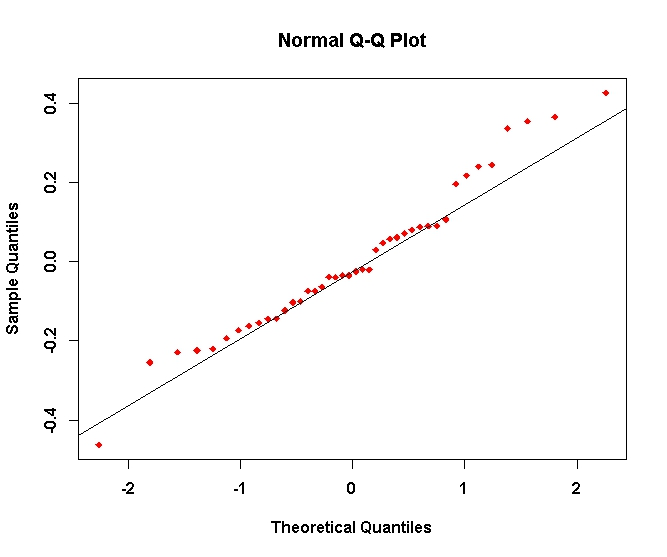
\includegraphics[scale=0.55]{images/ExamQ5qqplot}
\end{center}
\begin{center}
	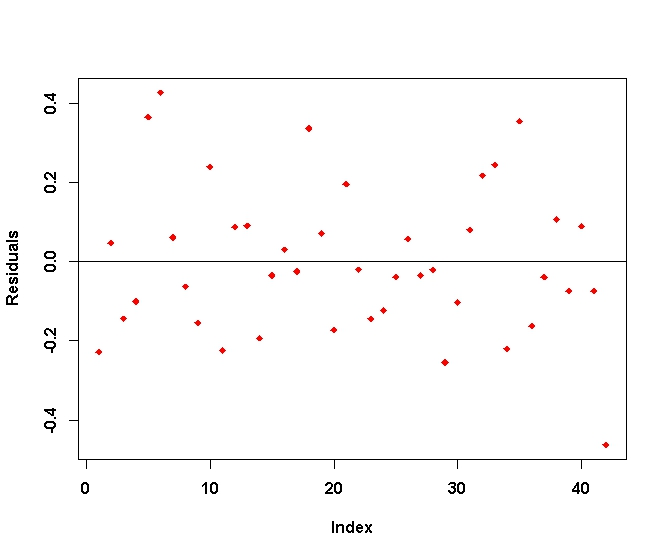
\includegraphics[scale=0.55]{images/ExamQ5resid}
\end{center}
\newpage



\subsection*{Question 39 - Control Charts Arithmetic}
A normally distributed quality characteristic is monitored through the use of control charts. These charts have the following parameters. All charts are in control.
\begin{center}
	\begin{tabular}{|c|c|c|c|}
		\hline  & LCL & Centre Line & UCL \\
		\hline $\bar{X}$-Chart & 614 & 620 & 626 \\
		\hline $R$-Chart & 0 & 8.236 & 18.795 \\ \hline
	\end{tabular}
\end{center}

\begin{itemize}
	\item[i.] (2 marks) What sample size is being used for this analysis?
	\item[ii.] (2 marks) Estimate the mean of the standard deviations $\bar{s}$ for this process.
	\item[iii.] (2 marks) Compute the control limits for the process standard deviation chart (i.e. the s-chart).
\end{itemize}

\subsection*{Question 40 - Process Capability Indices}

An automobile assembly plant concerned about quality improvement measured sets of five camshafts on twenty occasions throughout the day. The specifications for the process state that the design specification limits at 600$\pm$3mm.


\begin{itemize}
	\item[i.] (2 marks) Determine the \emph{Process Capability Indices} $C_p$ and $C_{pk}$, commenting on the respective values. You may use the \texttt{R} code output on the following page.
	\item[ii.] (2 marks)  The value of $C_{pm}$ is $1.353$. Explain why there would be a discrepancy between $C_p$ and $C_{pm}$.
	\item[iii.] (2 marks) Comment on the graphical output of the \emph{Process Capability Analysis}, also presented on the next page.
\end{itemize}


\newpage
\begin{framed}
	\begin{verbatim}
	Process Capability Analysis
	
	Call:
	process.capability(object = obj, spec.limits = c(597, 603))
	Number of obs = 100          Target = 600
	Center = 599.548         LSL = 597
	StdDev = 0.5846948       USL = 603
	
	Capability indices:
	Value   2.5%  97.5%
	Cp    ...
	Cp_l  ...
	Cp_u  ...
	Cp_k  ...
	Cpm   1.353  1.134  1.572
	Exp<LSL 0%   Obs<LSL 0%
	\end{verbatim}
\end{framed}



\begin{center}
	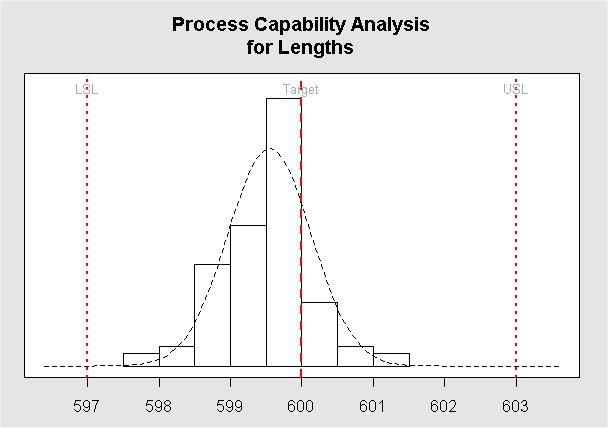
\includegraphics[scale=0.55]{images/ExamQ4hist}
\end{center}
\newpage
%
%Lengths = Values
%
%obj <- qcc(Lengths, type="xbar")
%
%process.capability(obj, spec.limits=c(597,603))

\subsection*{Question 41 - Statistical Process Control}
Answer the following questions.

\begin{itemize}
	\item[(i)] (1 marks) Differentiate common causes of variation in the quality of process output from assignable causes.
	\item[(ii.)] (1 marks) What is tampering in the context of statistical process control?
	\item[(iii.)] (4 marks) Other than applying the \emph{Three Sigma} rule for detecting the presence of an assignable cause, what else do we look for when studying a control chart? Support your answer with sketches.
\end{itemize}
\textit{(Remark - Part (iii) of this question is similar to Question 47. Question 47 prompts you discuss the probabilities more.)}
\subsection*{Question 42 - Control Charts Arithmetic}

A normally distributed quality characteristic is monitored through the use of control charts. These charts have the following parameters. All charts are in control.
\begin{center}
	\begin{tabular}{|c|c|c|c|}
		\hline  & LCL & Centre Line & UCL \\
		\hline $\bar{X}$-Chart & 542 & 550 & 558 \\
		\hline $R$-Chart & 0 & 8.236 & 16.504 \\ \hline
	\end{tabular}
\end{center}

\begin{itemize}
	\item[(i.)] (2 marks) What sample size is being used for this analysis?
	\item[(ii.)](2 marks) Estimate the mean of the standard deviations $\bar{s}$ for this process.
	\item[(iii.)] (2 marks) Compute the control limits for the process standard deviation chart (i.e. the s-chart).
\end{itemize}

\subsection*{Question 43 - Process Capability Indices} 

An automobile assembly plant concerned about quality improvement measured sets of five camshafts on twenty occasions throughout the day. The specifications for the process state that the design specification limits at 600$\pm$3mm.


\begin{itemize}
	\item[i.] (4 marks) Determine the \emph{Process Capability Indices} $C_p$ and $C_{pk}$, commenting on the respective values. You may use the \texttt{R} code output on the following page.
	\item[ii.] (2 marks)  The value of $C_{pm}$ is $1.353$. Explain why there would be a discrepancy between $C_p$ and $C_{pm}$.
	\item[iii.] (2 marks) Comment on the graphical output of the \emph{Process Capability Analysis}, also presented on the next page.
\end{itemize}


\newpage
\begin{framed}
	\begin{verbatim}
	Process Capability Analysis
	
	Call:
	process.capability(object = obj, spec.limits = c(597, 603))
	Number of obs = 100          Target = 600
	Center = 599.548         LSL = 597
	StdDev = 0.5846948       USL = 603
	
	Capability indices:
	Value   2.5%  97.5%
	Cp    ...
	Cp_l  ...
	Cp_u  ...
	Cp_k  ...
	Cpm   1.353  1.134  1.572
	Exp<LSL 0%   Obs<LSL 0%
	\end{verbatim}
\end{framed}



\begin{center}
	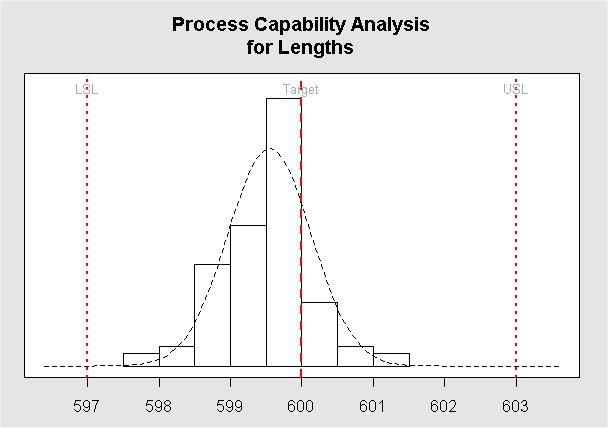
\includegraphics[scale=0.55]{images/ExamQ4hist}
\end{center}
\newpage
%
%Lengths = Values
%
%obj <- qcc(Lengths, type="xbar")
%
%process.capability(obj, spec.limits=c(597,603))
\subsection*{Question 44 - Factorial Design}
An experiment is run on an operating chemical process in which the aim is to reduce the
amount of impurity produced. Three continuous variables are thought to affect impurity,
these are concentration of NaOH, agitation speed and temperature. As an initial investigation two settings are selected for each variable these are

\begin{center}
	\begin{tabular}{|c|c|c|}
		\hline
		% after \\: \hline or \cline{col1-col2} \cline{col3-col4} ...
		Factor: &low level & highlevel  \\ \hline
		Concentration of NaOH & $40\%$ & $45\%$\\
		Agitation speed (rpm) & 15 & 25 \\
		Temperature ($^{\circ}{\rm F}$) & 170 & 200 \\
		\hline
	\end{tabular}
\end{center}
Readings were recorded of the impurity produced from the chemical process for each combination of the levels of these factors, and each combination was tested twice.
\begin{center}
	\begin{tabular}{|c|c|c|c|}
		\hline
		% after \\: \hline or \cline{col1-col2} \cline{col3-col4} ...
		Conc NaOH & Agitation & Temperature & Impurity \\
		-	&	-	&	-	&	 90,70	\\
		+	&	-	&	-	&    100,120	\\
		-	&	+	&	-	&	 90,110	\\
		+	&	+	&	-	&	 120,150	\\
		-	&	-	&	+	&	 110,100\\
		+	&	-	&	+	&	 100,130	\\
		-	&	+	&	+	&	 100,80	\\
		+	&	+	&	+	&	 160,140\\
		\hline
	\end{tabular}
\end{center}
\begin{itemize}
	\item[i.] (8 Marks) Calculate the contrasts, the effects and the sum of squares for the effects.
	\item[ii.] (8 Marks) Using the computed sums of squares values, complete the ANOVA table (see the \texttt{R} code below).
	\item[iii.] (4 Marks) Comment on the tests for significant for the main effects and interactions. State clearly your conclusions.
	\item[iv.] (4 Marks) Write down a  regression equation that can be used predicting impurity based on the results of this experiment.
\end{itemize}

\begin{framed}
	\begin{verbatim}
	Df Sum Sq Mean Sq F value  Pr(>F)
	Conc            1    ...     ...   ...   0.00253 **
	Agit            1    ...     ...   ...   0.07093 .
	Temp            1    ...     ...   ...   0.29485
	Conc:Agit       1    ...     ...   ...   0.48239
	Conc:Temp       1    ...     ...   ...   0.87675
	Agit:Temp       1    ...     ...   ...   0.44646
	Conc:Agit:Temp  1    ...     ...   ...   0.18751
	Residuals       8   1950     244
	\end{verbatim}
\end{framed}

\newpage
\begin{center}
	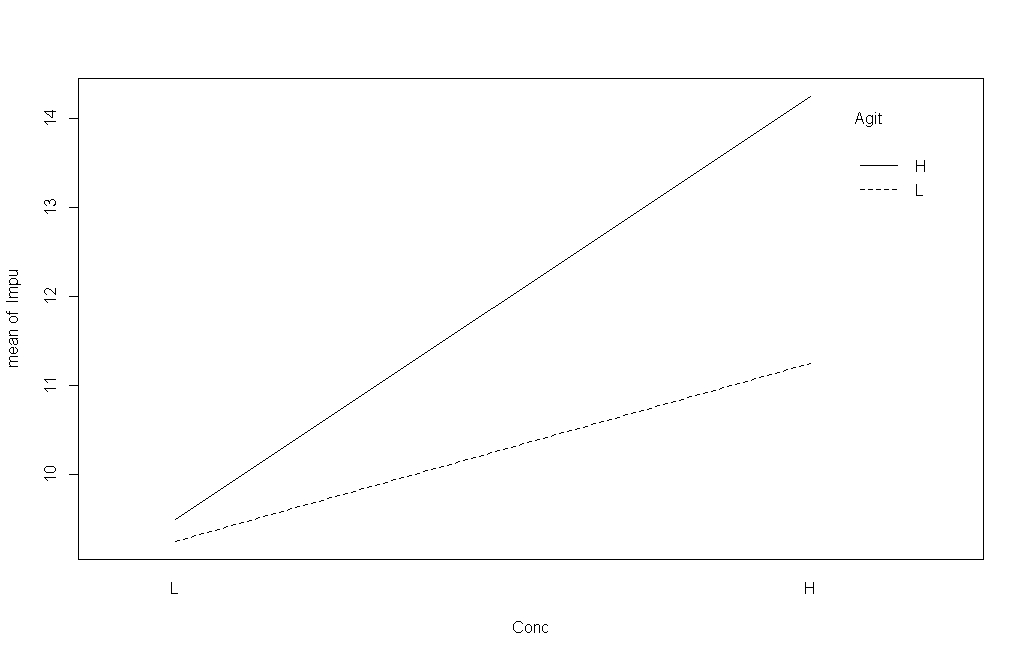
\includegraphics[scale=0.3]{image/ExamQ6interactiona}
\end{center}
\begin{center}
	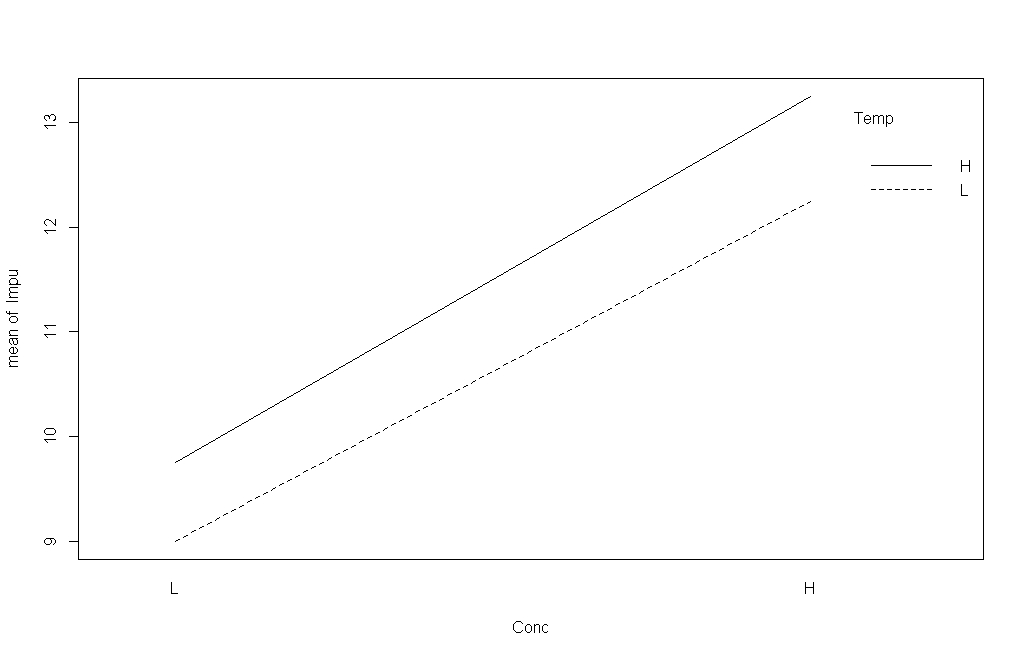
\includegraphics[scale=0.3]{image/ExamQ6interactionb}
\end{center}
\begin{center}
	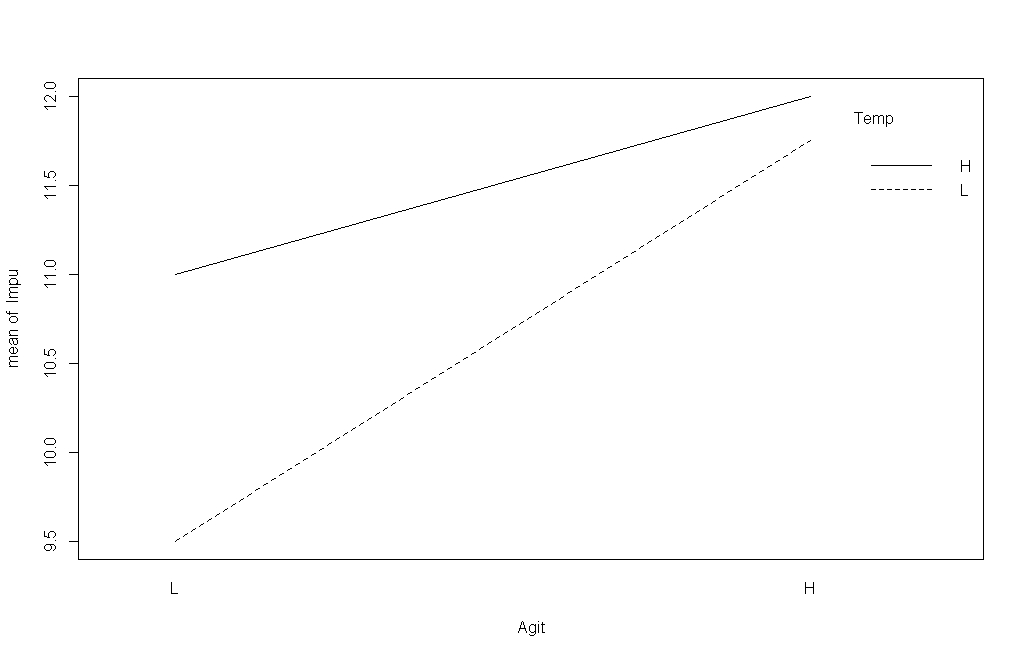
\includegraphics[scale=0.3]{image/ExamQ6interactionc}
\end{center}

\newpage
\subsection*{Question 45 - Statistical Process Control}
Answer the following questions.

\begin{itemize}
	\item[i.] (1 marks) What is the purpose of maintaining control charts?
	\item[ii.] (1 marks) What is the \emph{\textbf{Three Sigma}} rule in the context of statistical process control?
%	\item[iii.] (4 marks) Other than applying the \emph{Three Sigma} rule for detecting the presence of an assignable cause, what else do we look for when studying a control chart? Limit your answer to three examples. Support your answer with sketches.
	\item[iii.] (2 Marks) What is a CUSUM chart? What type of departures from the production target value
	is this type of chart useful for detecting?
\end{itemize}


\newpage
\subsection*{Question 46 - Regression Analysis}
\begin{figure}[h!]
	\centering
	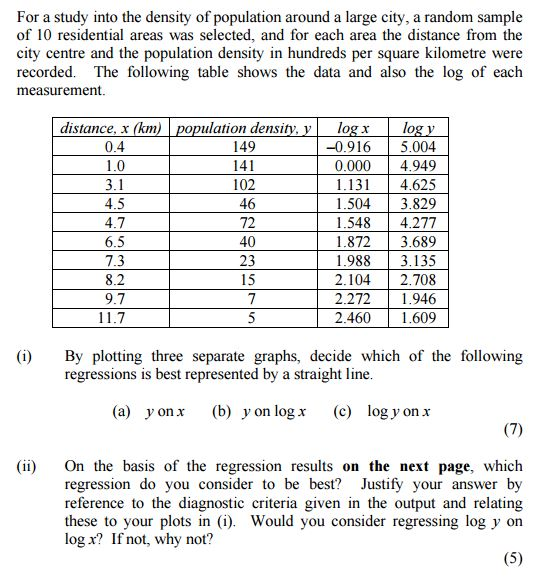
\includegraphics[width=0.8\linewidth]{images/ReviewQ18-a}
\end{figure}
\begin{figure}[h!]
	\centering
	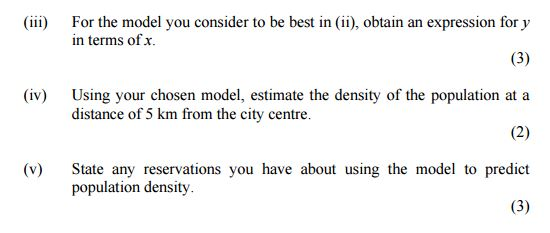
\includegraphics[width=0.8\linewidth]{images/ReviewQ18-b}
\end{figure}
\newpage
\begin{figure}[h!]
	\centering
	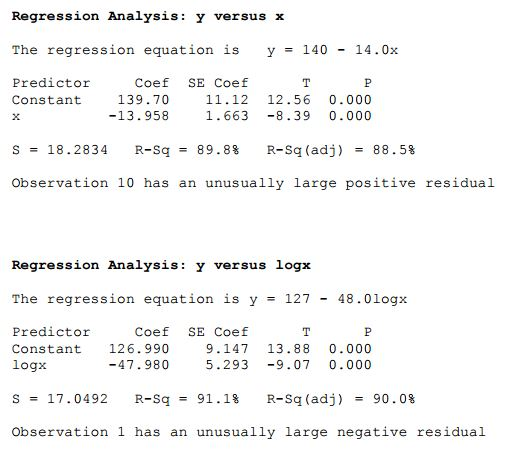
\includegraphics[width=0.8\linewidth]{images/ReviewQ18-c}
\end{figure}
\begin{figure}[h!]
	\centering
	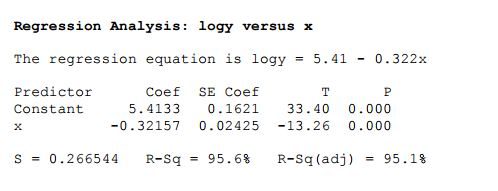
\includegraphics[width=0.8\linewidth]{images/ReviewQ18-d}
\end{figure}

\newpage

\subsection*{Question 47 - Nelson Rules for Control Charts}
The \textbf{Nelson Rules} are a set of eight decision rules for detecting ``out-of-control" or non-random conditions on control charts. These rules are applied to a control chart on which the magnitude of some variable is plotted against time. The rules are based on the mean value and the standard deviation of the samples.\\

\begin{itemize}
\item[(i)] ($4 \times 2$ Marks) Discuss any four of these rules, and how they would be used to detect ``out of control" processes. Support your answer with sketch.
\end{itemize}

\bigskip 
\begin{framed}
\noindent \textit{In your answer, you may make reference to the following properties of the Normal Distribution. Consider the random variable $X$ distributed as
\[X \sim \mathcal{N}(\mu,\sigma^2)\]
where $\mu$ is the mean and $\sigma^2$ is the variance of an random variable $X$.}
\begin{itemize}
	\item $\Pr( \mu - 1\sigma \leq X \leq \mu + 1\sigma ) = 0.6827$
	\item $\Pr( \mu - 2\sigma \leq X \leq \mu + 2\sigma ) = 0.9545$
	\item $\Pr( \mu - 3\sigma \leq X \leq \mu + 3\sigma )= 0.9973$
	
\end{itemize}
\end{framed}

%\subsection*{Question 48 - Tukey's Ladder For Data Transformation}
%\begin{itemize}
%%	\item Describe the purpose of transformations
%%	\item Describe the process of transformations
%	\item[(i)](1 Mark) Describe the purpose of Tukey's Ladder (referencing direction and relative strength)
%	\item[(ii)] (2 Marks) Give an example of a transformation for various types of skewed data (use Tukey's Ladder, with an example for both directions)
%	\item[(iii)] (2 Marks) Describe the limitations of transformations
%\end{itemize}	
\newpage
\subsection*{Question 48 - Method of Standard Additions}
Short Question on Method of Standard Additions. For 2015 - you should expect nothing more than a general theory question on the idea behind it.
\subsection*{Question 49 - Limits of Detection}
Short Question on Limits of Detection. Expect a calculation question. You will \textbf{not} be given the formula.
\[\mbox{LoD} = Y_B + 3S_B\]
From the R code output you will be given an indication to use the intercept  as $Y_B$ and  Residual Standard Error  as the $S_B$ %
\begin{figure}[h!]
\centering
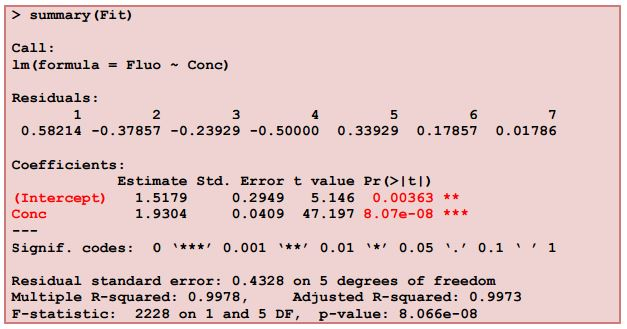
\includegraphics[width=1.1\linewidth]{image/LoD}
\caption{}
\label{fig:LoD}
\end{figure}

\newpage
\section*{Formulae and Tables}
\subsection*{Critical Values for Dixon Q Test}
{
	\Large
	\begin{center}
		\begin{tabular}{|c|c|c|c|}
			\hline  N  & $\alpha=0.10$  & $\alpha=0.05$  & $\alpha=0.01$  \\ \hline
			3  & 0.941 & 0.97  & 0.994 \\ \hline
			4  & 0.765 & 0.829 & 0.926 \\ \hline
			5  & 0.642 & 0.71  & 0.821 \\ \hline
			6  & 0.56  & 0.625 & 0.74  \\ \hline
			7  & 0.507 & 0.568 & 0.68  \\ \hline
			8  & 0.468 & 0.526 & 0.634 \\ \hline
			9  & 0.437 & 0.493 & 0.598 \\ \hline
			10 & 0.412 & 0.466 & 0.568 \\ \hline
			11 & 0.392 & 0.444 & 0.542 \\ \hline
			12 & 0.376 & 0.426 & 0.522 \\ \hline
			13 & 0.361 & 0.41  & 0.503 \\ \hline
			14 & 0.349 & 0.396 & 0.488 \\ \hline
			15 & 0.338 & 0.384 & 0.475 \\ \hline
			16 & 0.329 & 0.374 & 0.463 \\ \hline
		\end{tabular} 
	\end{center}
}
\subsection*{ANOVA Pocedures}
\[ \mbox{Var}(Y) = \frac{SS_{tot}}{n-1} \]
\subsection*{Two Way ANOVA}
\[ \textrm{MS}_{A} =  c \times S^2_{R} \phantom{space} (= \textrm{MS}_{Trt} )\]
\[ \textrm{MS}_{B} =  r \times S^2_{C} \phantom{space} (= \textrm{MS}_{Block})\]

\end{document}

\subsection*{Confidence Intervals}
{\bf One sample}
\begin{eqnarray*} S.E.(\bar{X})&=&\frac{\sigma}{\sqrt{n}}.\\\\
S.E.(\hat{P})&=&\sqrt{\frac{\hat{p}\times(100-\hat{p})}{n}}.\\
\end{eqnarray*}
{\bf Two samples}
\begin{eqnarray*}
S.E.(\bar{X}_1-\bar{X}_2)&=&\sqrt{\frac{\sigma^2_1}{n_1}+\frac{\sigma_2^2}{n_2}}.\\\\
S.E.(\hat{P_1}-\hat{P_2})&=&\sqrt{\frac{\hat{p}_1\times(100-\hat{p}_1)}{n_1}+\frac{\hat{p}_2\times(100-\hat{p}_2)}{n_2}}.\\\\
\end{eqnarray*}
\subsection*{Hypothesis tests}
{\bf One sample}
\begin{eqnarray*}
S.E.(\bar{X})&=&\frac{\sigma}{\sqrt{n}}.\\\\
S.E.(\pi)&=&\sqrt{\frac{\pi\times(100-\pi)}{n}}
\end{eqnarray*}
{\bf Two large independent samples}
\begin{eqnarray*}
S.E.(\bar{X}_1-\bar{X}_2)&=&\sqrt{\frac{\sigma^2_1}{n_1}+\frac{\sigma_2^2}{n_2}}.\\\\
S.E.(\hat{P_1}-\hat{P_2})&=&\sqrt{\left(\bar{p}\times(100-\bar{p})\right)\left(\frac{1}{n_1}+\frac{1}{n_2}\right)}.\\
\end{eqnarray*}
{\bf Two small independent samples}
\begin{eqnarray*}
S.E.(\bar{X}_1-\bar{X}_2)&=&\sqrt{s_p^2\left(\frac{1}{n_1}+\frac{1}{n_2}\right)}.\\\\
s_p^2&=&\frac{s_1^2(n_1-1)+s_2^2(n_2-1)}{n_1+n_2-2}.\\
\end{eqnarray*}
{\bf Paired sample}
\begin{eqnarray*}
S.E.(\bar{d})&=&\frac{s_d}{\sqrt{n}}.\\\\
\end{eqnarray*}
{\bf Standard Deviation of case-wise differences (computational formula)}
\begin{eqnarray*}
s_d = \sqrt{ {\sum d_i^2 - n\bar{d}^2 \over n-1}}.\\\\
\end{eqnarray*}
\end{document}
% -- Part 3 - Confidence Interval

% 2 Marks Using previously calculated values, compute the confidence interval
